% Author: Jan Schaumann <jschauma@netmeister.org>
% $Id: slides.tex,v 1.13 2005/03/14 21:41:25 jschauma Exp $

% CampusDomain!2011
\special{! TeXDict begin /landplus90{true}store end }

\documentclass[xga]{xdvislides}
\usepackage[landscape]{geometry}
\usepackage{graphics}
\usepackage{graphicx}
\usepackage{colordvi}
\usepackage{multirow}

\usepackage{fancyvrb}
\fvset{commandchars=\\\{\}}

\usepackage[usenames]{color}
\definecolor{gray}{RGB}{180,180,180}

\newcommand{\smallish}{\fontsize{16}{16}\selectfont}

\begin{document}
\setfontphv

%%% Headers and footers
\lhead{\slidetitle}                               % default:\lhead{\slidetitle}
\chead{CS615 - Aspects of System Administration}% default:\chead{\relax}
\rhead{Slide \thepage}                       % default:\rhead{\sectiontitle}
\lfoot{\Gray{Networking II}}% default:\lfoot{\slideauthor}
\cfoot{\relax}                               % default:\cfoot{\relax}
\rfoot{\Gray{\today}}

\vspace*{\fill}
\begin{center}
	\Hugesize
		CS615 - Aspects of System Administration\\ [1em]
		Networking II\\ [1em]
	\hspace*{5mm}\blueline\\ [1em]
	\Normalsize
		Department of Computer Science\\
		Stevens Institute of Technology\\
		Jan Schaumann\\
		\verb+jschauma@stevens.edu+\\
		\verb+http://www.cs.stevens.edu/~jschauma/615A/+
\end{center}
\vspace*{\fill}

\subsection{Get your instruments and play along!}

\Hugesize
\vspace*{\fill}
Start a FreeBSD instance, then log in on it. \\

{\tt ami-d0b520b8 --instance-type t1.micro} \\

{\tt ssh ec2-user@<instance-name>}
\vspace*{\fill}
\Normalsize

\subsection{A simple example}
\Hugesize
\begin{center}
\begin{verbatim}
$ telnet www.google.com 80

\end{verbatim}
\end{center}
\Normalsize
\vspace*{\fill}

\subsection{A simple example}
\Hugesize
\begin{center}
\begin{verbatim}
$ telnet www.google.com 80
Trying 172.217.15.68...
Connected to www.google.com.
Escape character is '^]'.
HEAD / HTTP/1.0

\end{verbatim}
\end{center}
\Normalsize
\vspace*{\fill}

\subsection{A simple example}
\Hugesize
\begin{center}
\begin{verbatim}
$ telnet www.google.com 80
Trying 172.217.15.68...
Connected to www.google.com.
Escape character is '^]'.
HEAD / HTTP/1.0

HTTP/1.0 200 OK
Date: Sun, 25 Feb 2018 18:18:45 GMT
Content-Type: text/html; charset=ISO-8859-1
Server: gws
[...]
\end{verbatim}
\end{center}
\Normalsize
\vspace*{\fill}

\subsection{A simple example}
What exactly happens?

\subsection{A simple example}
What exactly happens?
\\
\begin{itemize}
	\item local host connects to remote host
	\item sends command
	\item receives data
\end{itemize}

\subsection{A simple example}
How exactly do we connect to the remote host?
\\
\begin{itemize}
	\item look up hostname
	\item open connection to IP address
\end{itemize}

\subsection{A simple example}
How exactly do we look up a hostname?

\subsection{A simple example}
\\
\Hugesize
\begin{center}
\begin{verbatim}
$ ktrace -i telnet www.google.com 80
Trying 172.217.15.68...
Connected to www.google.com.
Escape character is '^]'.
GET / HTTP/1.0

[...]
$ kdump >trace
\end{verbatim}
\end{center}
\Normalsize
\vspace*{\fill}

\subsection{...open a few files...}
\smallish
\begin{verbatim}
[...]
   735 ktrace   RET   execve -1 errno 2 No such file or directory
   735 ktrace   CALL  execve(0xbfbfe7e0,0xbfbfed00,0xbfbfed10)
   735 ktrace   NAMI  "/usr/bin/telnet"
   735 ktrace   NAMI  "/libexec/ld-elf.so.1"
   735 telnet   RET   execve 0
[...]
   735 telnet   CALL  open(0x285192e8,0x100000<O_CLOEXEC>,<unused>0x1b6)
   735 telnet   NAMI  "/etc/nsswitch.conf"
   735 telnet   RET   open 3
[...]
   735 telnet   CALL  open(0x285172f5,0x100000<O_CLOEXEC>,<unused>0x1b6)
   735 telnet   NAMI  "/etc/hosts"
   735 telnet   RET   open 3
[...]
   735 telnet   CALL  open(0x28516f79,0x100000<O_CLOEXEC>,<unused>0x1b6)
   735 telnet   NAMI  "/etc/resolv.conf"
   735 telnet   RET   open 3
[...]
   735 telnet   CALL  read(0x3,0x28c31000,0x8000)
   735 telnet   GIO   fd 3 read 70 bytes
       "# Generated by resolvconf
        search ec2.internal
        nameserver 172.16.0.23
\end{verbatim}
\Normalsize

\subsection{... query a DNS server ...}
\smallish
\begin{verbatim}
[...]
   735 telnet   CALL  socket(PF_INET,SOCK_CLOEXEC|SOCK_DGRAM,IPPROTO_IP)
   735 telnet   RET   socket 4
   735 telnet   CALL  connect(0x4,0x28547e64,0x10)
   735 telnet   STRU  struct sockaddr { AF_INET, 172.16.0.23:53 }
   735 telnet   RET   connect 0
   735 telnet   CALL  sendto(0x4,0x28c5f000,0x20,0,0,0)
   735 telnet   GIO   fd 4 wrote 32 bytes
       0x0000 9a70 0100 0001 0000 0000 0000 0377 7777 0667 6f6f 676c  |.p...........www.googl|
       0x0016 6503 636f 6d00 0001 0001                                |e.com.....|
[...]
   735 telnet   CALL  recvfrom(0x4,0x28c4f000,0x10000,0,0xbfbfd5d0,0xbfbfd5cc)
   735 telnet   GIO   fd 4 read 60 bytes
       0x0000 d6c6 8180 0001 0001 0000 0000 0377 7777 0667 6f6f 676c  |.............www.googl|
       0x0016 6503 636f 6d00 001c 0001 c00c 001c 0001 0000 003c 0010  |e.com..............<..|
       0x002c 2607 f8b0 4004 0807 0000 0000 0000 2004                 |&...@......... .|
[...]
\end{verbatim}
\Normalsize

\subsection{A simple example}
How exactly do we look up a hostname?
\\
\begin{itemize}
	\item look up various local files
	\item open a connection to a DNS server's IP
	\item ask DNS server to resolve hostname
	\item get back IP
\end{itemize}
\vspace{.5in}

And then?

\subsection{...communicate with the remote host...}
\smallish
\begin{verbatim}
   735 telnet   GIO   fd 1 wrote 25 bytes
       "Trying 216.58.217.132...
       "
   735 telnet   RET   write 25/0x19
   735 telnet   CALL  socket(PF_INET,SOCK_STREAM,IPPROTO_TCP)
   735 telnet   CALL  connect(0x3,0x28c0f0f0,0x10)
   735 telnet   STRU  struct sockaddr { AF_INET, 216.58.217.132:80 }
[...]
   918 telnet   GIO   fd 0 read 16 bytes
       "HEAD / HTTP/1.0
       "
   918 telnet   RET   read 16/0x10
   918 telnet   CALL  select(0x4,0x28c0d1b8,0x28c0d1c0,0x28c0d1c8,0x80677b8)
   918 telnet   RET   select 1
   918 telnet   CALL  sendto(0x3,0x8068048,0x11,0,0,0)
   918 telnet   GIO   fd 3 wrote 17 bytes
       "HEAD / HTTP/1.0\r
       "
[...]
   918 telnet   RET   select 1
   918 telnet   CALL  recvfrom(0x3,0x8068870,0x400,0,0,0)
   918 telnet   GIO   fd 3 read 665 bytes
       "HTTP/1.0 200 OK\r
        Date: Sun, 25 Feb 2018 18:55:15 GMT\r
\end{verbatim}
\Normalsize

\subsection{Ok, so how does this work?}
\begin{itemize}
	\item determine which nameserver to query
	\item ask who has a route to the nameserver
	\item open socket to well defined port on remote IP
	\item send queries
	\item open socket to requested port on remote IP
\end{itemize}

\subsection{Let's collect some data...}
\begin{verbatim}
laptop$ ssh ec2-user@<instance-name>
$ su
# script commands.out
# ifconfig -a
# route -n get default
# cat /etc/resolv.conf
# tcpdump -w tcpdump.out port not 22 >&/dev/null &
# arp -d -a
# ping -n -c 3 8.8.8.8
# ktrace -i telnet www.google.com 80
HEAD / HTTP/1.0
# kill %1
# kdump > kdump.out
# exit
# exit
$ exit
laptop$ scp ec2-user@<instance-name>:*out /tmp/
\end{verbatim}

\subsection{A simple example}
Finding the next hop:
\begin{verbatim}
$ tcpdump -t -n -r /tmp/tcpdump.out arp
reading from file tcpdump.out, link-type EN10MB (Ethernet)
ARP, Request who-has 10.234.105.193 tell 10.234.105.225, length 28
ARP, Reply 10.234.105.193 is-at fe:ff:ff:ff:ff:ff, length 28
ARP, Request who-has 10.234.105.225 tell 10.234.105.193, length 28
ARP, Reply 10.234.105.225 is-at 22:00:0a:ea:69:e1, length 28
\end{verbatim}

\subsection{A simple example}
Performing the DNS query:
\begin{verbatim}
$ tcpdump -t -n -r tcpdump.out udp port 53
reading from file tcpdump.out, link-type EN10MB (Ethernet)
IP 10.234.105.225.12637 > 172.16.0.23.53: 32409+ A? www.google.com. (32)
IP 172.16.0.23.53 > 10.234.105.225.12637: 32409 1/0/0 A 172.217.12.228 (48)
IP 10.234.105.225.33347 > 172.16.0.23.53: 49414+ AAAA? www.google.com. (32)
IP 172.16.0.23.53 > 10.234.105.225.33347: 49414 1/0/0 AAAA 2607:f8b0:4004:807::2004 (60)
\end{verbatim}

\subsection{A simple example}
Establishing the connection to the server:
\begin{verbatim}
$ tcpdump -t -n -r tcpdump.out tcp port 80
IP 10.234.105.225.50194 > 172.217.15.68.80: Flags [S],
        seq 1054601677, win 65535, options [...], length 0
IP 172.217.15.68.80 > 10.234.105.225.50194: Flags [S.],
        seq 230054466, ack 1054601678, win 42408, options [...], length 0
IP 10.234.105.225.50194 > 172.217.15.68.80: Flags [.],
        ack 1, win 1026, options [...], length 0
\end{verbatim}

\subsection{A simple example}
Sending the HTTP request:
\begin{verbatim}
IP 10.234.105.225.50194 > 172.217.15.68.80: Flags [P.],
        seq 1:18, ack 1, win 1026, options [...], length 17
IP 172.217.15.68.80 > 10.234.105.225.50194: Flags [.],
        ack 18, win 166, options [...], length 0
IP 10.234.105.225.50194 > 172.217.15.68.80: Flags [P.],
        seq 18:20, ack 1, win 1026, options [...], length 2
IP 172.217.15.68.80 > 10.234.105.225.50194: Flags [.],
        ack 20, win 166, options [...], length 0
\end{verbatim}

\subsection{A simple example}
Receiving the HTTP response:
\begin{verbatim}
IP 172.217.15.68.80 > 10.234.105.225.50194: Flags [P.],
        seq 1:666, ack 20, win 166, options [...], length 665
IP 10.234.105.225.50194 > 172.217.15.68.80: Flags [.],
        ack 667, win 1015, options [...], length 0
\end{verbatim}

\subsection{A simple example}
Terminating the connection:
\begin{verbatim}
IP 172.217.15.68.80 > 10.234.105.225.50194: Flags [F.],
        seq 666, ack 20, win 166, options [...], length 0
IP 10.234.105.225.50194 > 172.217.15.68.80: Flags [F.],
        seq 20, ack 667, win 1026, options [...], length 0
IP 172.217.15.68.80 > 10.234.105.225.50194: Flags [.],
        ack 21, win 166, options [...], length 0
\end{verbatim}

\subsection{Notables from this simple example}
``Simple'' is, as usual, relative.

\subsection{Notables from this simple example}
``Simple'' is, as usual, relative.
\\

\begin{itemize}
	\item host configuration assumed
	\item network architecture (internal or across the internet) not
			relevant (here)
	\item even simple examples cross multiple layers and protocols
			(HTTP, DNS; TCP, UDP, ARP)
	\item we haven't even scratched the surface
\end{itemize}

\subsection{TCP/IP Basics: Protocol Layers}
\begin{center}
	\begin{tabular}{|cl|l|}
	\hline
	& {\bf Layer} & {\bf Function} \\
	\hline
	4. & Application Layer & End-User application programs \\
	3. & Transport Layer & Delivery of data to applications \\
	2. & Network Layer & Basic communication, addressing, and routing \\
	\multirow{2}{*}{1.} & Link Layer & Network Hardware and device drivers \\
	& Physical Layer & Cable or physical medium \\
	\hline
	\end{tabular}
\end{center}
\addvspace{.5in}
Examples of protocols for each layer:
\begin{itemize}
	\item Simple Mail Transfer Protocol (RFC 821) \\
		Hypertext Transfer Protocol (RFC 2616)
	\item Transmission Control Protocol (RFC 793, tcp(4)) \\
		User Datagram Protocol (RFC 768; udp(4))
	\item Internet Protocol (RFC 791; ip(4)) \\
		Internet Control Message Protocol (RFC 792; icmp(4))
	\item Address Resolution Protocol (RFC 826; arp(4))
\end{itemize}

\subsection{TCP/IP Basics: Protocol Layers (OSI Model)}
\vspace*{\fill}
\begin{center}
	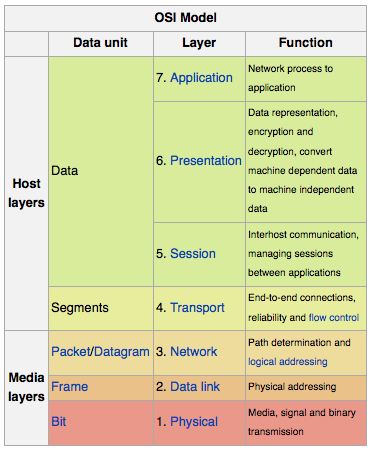
\includegraphics[scale=0.7]{pics/osi.eps}
\end{center}
\vspace*{\fill}

\subsection{TCP/IP Basics: ARP}
\begin{center}
Ethernet Address Resolution Protocol \\
-- or -- \\
Converting Network Protocol Addresses to 48-bit Ethernet Address for Transmission on Ethernet Hardware
\end{center}

\begin{verbatim}
$ arp -a
falcon.srcit.stevens-tech.edu (155.246.89.89) at 00:07:e9:09:ca:10 [ether] on eth0
grohl.srcit.stevens-tech.edu (155.246.89.9) at 00:16:3e:cf:6b:5b [ether] on eth0
hoth.srcit.stevens-tech.edu (155.246.89.10) at 00:1e:68:8e:79:d8 [ether] on eth0
cinema.srcit.stevens-tech.edu (155.246.89.67) at 00:25:90:1e:05:51 [ether] on eth0
vlan16.cc.stevens-tech.edu (155.246.89.1) at 00:00:5e:00:01:02 [ether] on eth0
vader.srcit.stevens-tech.edu (155.246.89.5) at 00:23:8b:a9:dd:60 [ether] on eth0
nirvana.phy.stevens-tech.edu (155.246.89.33) at 00:1e:68:0f:99:a2 [ether] on eth0
\end{verbatim}

\subsection{TCP/IP Basics: ARP}
\vspace*{\fill}
\begin{center}
	\includegraphics[scale=0.8]{pics/3computers-arp.eps}
\end{center}
\vspace*{\fill}


\subsection{TCP/IP Basics: ARP}
\begin{center}
Ethernet Address Resolution Protocol \\
-- or -- \\
Converting Network Protocol Addresses to 48-bit Ethernet Address for Transmission on Ethernet Hardware
\end{center}
\vspace{.2in}

\begin{verbatim}
ARP, Request who-has 10.114.62.1 tell 10.114.63.209, length 28
ARP, Reply 10.114.62.1 is-at fe:ff:ff:ff:ff:ff, length 28
ARP, Request who-has 10.114.63.209 (ff:ff:ff:ff:ff:ff) tell 0.0.0.0, length 28
ARP, Reply 10.114.63.209 is-at 12:31:3d:04:30:23, length 28
ARP, Request who-has 10.114.63.209 (ff:ff:ff:ff:ff:ff) tell 0.0.0.0, length 28
ARP, Reply 10.114.63.209 is-at 12:31:3d:04:30:23, length 28
ARP, Request who-has 10.114.63.209 (ff:ff:ff:ff:ff:ff) tell 0.0.0.0, length 28
ARP, Reply 10.114.63.209 is-at 12:31:3d:04:30:23, length 28
\end{verbatim}

\subsection{TCP/IP Basics: ND}
\begin{center}
Neighbor Discovery Protocol
\end{center}
\vspace{.2in}

\begin{verbatim}
$ ndp -n -a
Neighbor                            Linklayer Address  Netif Expire      S Flags
2001:470:30:84:e276:63ff:fe72:3900  e0:76:63:72:39:00  xennet0 permanent R
fe80::21b:21ff:fe45:bf54%xennet0    00:1b:21:45:bf:54  xennet0 21m52s    S R
fe80::21b:21ff:fe7a:7269%xennet0    00:1b:21:7a:72:69  xennet0 23h59m59s S R
fe80::e276:63ff:fe72:3900%xennet0   e0:76:63:72:39:00  xennet0 permanent R
fe80::1%lo0                          (incomplete)      lo0     permanent R
$
\end{verbatim}

\subsection{TCP/IP Basics: ND}
\begin{center}
Neighbor Discovery Protocol
\end{center}
\vspace{.2in}
\begin{verbatim}
IP6 fe80::21b:21ff:fe7a:7269 > ff02::1:ff62:3400: ICMP6,
        neighbor solicitation, who has 2001:470:30:84:e276:63ff:fe62:3400, length 32
IP6 2001:470:30:84:e276:63ff:fe72:3900 > ff02::1:ff7a:7269: ICMP6,
        neighbor solicitation, who has fe80::21b:21ff:fe7a:7269, length 32
IP6 fe80::21b:21ff:fe7a:7269 > 2001:470:30:84:e276:63ff:fe72:3900:
        ICMP6, neighbor advertisement, tgt is fe80::21b:21ff:fe7a:7269, length 32
\end{verbatim}

\subsection{TCP/IP Basics: ICMP}
\begin{center}
Internet Control Message Protocol
\end{center}
\vspace{.2in}

\begin{verbatim}
$ ping -c 3 www.yahoo.com
PING any-fp.wa1.b.yahoo.com (67.195.160.76): 56 data bytes
64 bytes from 67.195.160.76: icmp_seq=0 ttl=53 time=30.888 ms
64 bytes from 67.195.160.76: icmp_seq=1 ttl=53 time=23.193 ms
64 bytes from 67.195.160.76: icmp_seq=2 ttl=53 time=25.433 ms

----any-fp.wa1.b.yahoo.com PING Statistics----
3 packets transmitted, 3 packets received, 0.0% packet loss
round-trip min/avg/max/stddev = 23.193/26.505/30.888/3.958 ms
$
\end{verbatim}

\subsection{TCP/IP Basics: ICMP: Ping}
\vspace*{\fill}
\begin{center}
	\includegraphics[scale=0.8]{pics/3computers-ping.eps}
\end{center}
\vspace*{\fill}


\subsection{TCP/IP Basics: ICMP}
\begin{center}
Internet Control Message Protocol
\end{center}
\vspace{.2in}

\begin{verbatim}
$ tcpdump -r tcpdump.out -n icmp
IP 10.234.84.220 > 207.237.69.79: ICMP echo request
IP 207.237.69.79 > 10.234.84.220: ICMP echo reply
IP 10.234.84.220 > 207.237.69.79: ICMP echo request
IP 207.237.69.79 > 10.234.84.220: ICMP echo reply
IP 10.234.84.220 > 207.237.69.79: ICMP echo request
IP 207.237.69.79 > 10.234.84.220: ICMP echo reply
\end{verbatim}


\subsection{TCP/IP Basics: ICMP6}
\begin{center}
Internet Control Message Protocol for IPv6
\end{center}
\vspace{.2in}

\begin{verbatim}
$ ping6 -c 3 www.netbsd.org
PING6(56=40+8+8 bytes) 2001:470:30:84:204:d7b0:0:1 -->
                       2001:4f8:3:7:2e0:81ff:fe52:9a6b
16 bytes from 2001:4f8:3:7:2e0:81ff:fe52:9a6b, icmp_seq=0 hlim=57 time=74.316 ms
16 bytes from 2001:4f8:3:7:2e0:81ff:fe52:9a6b, icmp_seq=1 hlim=57 time=71.260 ms
16 bytes from 2001:4f8:3:7:2e0:81ff:fe52:9a6b, icmp_seq=2 hlim=57 time=71.321 ms

--- www.netbsd.org ping6 statistics ---
3 packets transmitted, 3 packets received, 0.0% packet loss
round-trip min/avg/max/std-dev = 71.260/72.299/74.316/1.747 ms
\end{verbatim}

\subsection{TCP/IP Basics: ICMP6}
\begin{center}
Internet Control Message Protocol for IPv6
\end{center}
\vspace{.2in}

\begin{verbatim}
IP6 2001:470:30:84:204:d7b0:0:1 >
   2001:4f8:3:7:2e0:81ff:fe52:9a6b: ICMP6, echo reque st, seq 0, length 16
IP6 2001:4f8:3:7:2e0:81ff:fe52:9a6b >
   2001:470:30:84:204:d7b0:0:1: ICMP6, echo reply , seq 0, length 16
IP6 2001:470:30:84:204:d7b0:0:1 >
   2001:4f8:3:7:2e0:81ff:fe52:9a6b: ICMP6, echo request, seq 1, length 16
IP6 2001:4f8:3:7:2e0:81ff:fe52:9a6b >
   2001:470:30:84:204:d7b0:0:1: ICMP6, echo reply , seq 1, length 16
IP6 2001:470:30:84:204:d7b0:0:1 >
   2001:4f8:3:7:2e0:81ff:fe52:9a6b: ICMP6, echo reque st, seq 2, length 16
IP6 2001:4f8:3:7:2e0:81ff:fe52:9a6b >
   2001:470:30:84:204:d7b0:0:1: ICMP6, echo reply , seq 2, length 16
\end{verbatim}

\subsection{TCP/IP Basics: ICMP: Traceroute}
\vspace*{\fill}
\begin{center}
	\includegraphics[scale=0.8]{pics/traceroute1.eps}
\end{center}
\vspace*{\fill}

\subsection{TCP/IP Basics: ICMP: Traceroute}
\vspace*{\fill}
\begin{center}
	\includegraphics[scale=0.8]{pics/traceroute2.eps}
\end{center}
\vspace*{\fill}

\subsection{TCP/IP Basics: ICMP: Traceroute}
\vspace*{\fill}
\begin{center}
	\includegraphics[scale=0.8]{pics/traceroute3.eps}
\end{center}
\vspace*{\fill}

\subsection{TCP/IP Basics: ICMP: Traceroute}
\vspace*{\fill}
\begin{center}
	\includegraphics[scale=0.8]{pics/traceroute4.eps}
\end{center}
\vspace*{\fill}



\subsection{TCP/IP Basics: ICMP}
\begin{center}
Internet Control Message Protocol
\end{center}
\vspace{.2in}

\begin{verbatim}
$ traceroute www.netbsd.org
traceroute to www.netbsd.org (204.152.190.12), 64 hops max, 40 byte packets
 1  eth2-3a.core1.nav.nyc.access.net (166.84.0.1)  0.256 ms  0.165 ms 0.181 ms
 2  l3v1.nyc.access.net (166.84.66.14)  1.570 ms  1.556 ms  1.437 ms
 3  gige-g3-3.core1.nyc4.he.net (209.51.171.25)  4.963 ms  2.422 ms  1.457 ms
 4  10gigabitethernet2-3.core1.ash1.he.net (72.52.92.86)  8.423 ms  8.769 ms  7.683 ms
 5  10gigabitethernet1-2.core1.atl1.he.net (184.105.213.110)  21.898 ms 19.647 ms  19.838 ms
 6  isc.gige-g2-1.core1.atl1.he.net (216.66.0.50)  77.465 ms  77.921 ms 80.519 ms
 7  iana.r1.atl1.isc.org (199.6.12.1)  77.302 ms  78.230 ms  81.782 ms
 8  int-0-5-0-1.r1.pao1.isc.org (149.20.65.37)  81.860 ms  83.780 ms 84.160 ms
 9  int-0-0-1-0.r1.sql1.isc.org (149.20.65.10)  81.543 ms  80.193 ms 84.434 ms
10  www.netbsd.org (204.152.190.12)  81.986 ms  81.008 ms  82.604 ms
$
\end{verbatim}

\subsection{TCP/IP Basics: ICMP}
\begin{center}
Internet Control Message Protocol
\end{center}

\begin{verbatim}
IP (tos 0x0, ttl 1, id 44866, offset 0, flags [none], proto UDP (17), length 40)
    166.84.7.99.44865 > 149.20.53.86.33435: [udp sum ok] UDP, length 12
IP (tos 0xc0, ttl 64, id 48796, offset 0, flags [none], proto ICMP (1), length 68)
    166.84.0.1 > 166.84.7.99: ICMP time exceeded in-transit, length 48
IP (tos 0x0, ttl 2, id 44869, offset 0, flags [none], proto UDP (17), length 40)
    166.84.7.99.44865 > 149.20.53.86.33438: [udp sum ok] UDP, length 12
IP (tos 0x0, ttl 3, id 44872, offset 0, flags [none], proto UDP (17), length 40)
    166.84.7.99.44865 > 149.20.53.86.33441: [udp sum ok] UDP, length 12
IP (tos 0x0, ttl 4, id 44875, offset 0, flags [none], proto UDP (17), length 40)
    166.84.7.99.44865 > 149.20.53.86.33444: [udp sum ok] UDP, length 12
IP (tos 0x0, ttl 252, id 6760, offset 0, flags [none], proto ICMP (1), length 56)
    154.24.25.109 > 166.84.7.99: ICMP time exceeded in-transit, length 36
...
IP (tos 0x0, ttl 248, id 0, offset 0, flags [none], proto ICMP (1), length 56)
    149.20.53.86 > 166.84.7.99: ICMP 149.20.53.86 udp port 33482 unreachable, length 36
\end{verbatim}


\subsection{TCP/IP Basics: ICMP6}
\begin{center}
Internet Control Message Protocol for IPv6
\end{center}
\vspace{.2in}

\begin{verbatim}
$ traceroute6 www.netbsd.org
traceroute6 to www.netbsd.org (2001:4f8:3:7:2e0:81ff:fe52:9a6b) from
    2001:470:30:84:204:d7b0:0:1, 64 hops max, 12 byte packets
 1  router.vc.panix.com  0.271 ms  0.282 ms  0.155 ms
 2  2001:470:30::a654:420e  5.459 ms  1.251 ms  1.073 ms
 3  gige-g3-3.core1.nyc4.he.net  1.288 ms  2.001 ms  10.176 ms
 4  10gigabitethernet8-3.core1.chi1.he.net  26.603 ms  20.532 ms  25.029 ms
 5  2001:470:1:34::2  72.033 ms  72.377 ms  72.686 ms
 6  iana.r1.ord1.isc.org  76.288 ms  72.773 ms  71.481 ms
 7  int-0-0-1-8.r1.pao1.isc.org  73.027 ms  76.489 ms  77.507 ms
 8  int-0-0-1-0.r2.sql1.isc.org  73.555 ms  75.367 ms  74.769 ms
 9  www.NetBSD.org  72.036 ms  72.522 ms  71.39 ms
$
\end{verbatim}

\subsection{TCP/IP Basics: ICMP6}
\begin{center}
Internet Control Message Protocol for IPv6
\end{center}

\begin{verbatim}
IP6 2001:470:30:84:204:d7b0:0:1.51749 >
        2001:4f8:3:7:2e0:81ff:fe52:9a6b.33435: UDP, length 12
IP6 2001:470:30:84::3 > 2001:470:30:84:204:d7b0:0:1:
        ICMP6, time exceeded in-transit [|icmp6]
IP6 2001:470:30:84:204:d7b0:0:1.51749 >
        2001:4f8:3:7:2e0:81ff:fe52:9a6b.33436: UDP, length 12
[...]
IP6 2001:470:30:84:204:d7b0:0:1.51749 >
        2001:4f8:3:7:2e0:81ff:fe52:9a6b.33461: UDP, length 12
IP6 2001:4f8:3:7:2e0:81ff:fe52:9a6b >
        2001:470:30:84:204:d7b0:0:1: ICMP6, destination unreachable[|icmp6]
\end{verbatim}

\subsection{TCP/IP Basics: TCP}
\begin{center}
Transmission Control Protocol
\end{center}
\vspace{.2in}
\begin{verbatim}
$ telnet www.google.com 80
Trying 173.194.73.99...
Connected to www.google.com.
Escape character is '^]'.
GET / HTTP/1.0

\end{verbatim}

\subsection{TCP/IP Basics: TCP}
\begin{center}
Transmission Control Protocol
\end{center}
\vspace{.2in}
\begin{verbatim}
IP 166.84.7.99.58356 > 67.195.160.76.80: S
      2267539609:2267539609(0) win 32768
      <mss 1460,nop,wscale 3,sackOK,nop,nop,nop,nop,timestamp 10>
IP 67.195.160.76.80 > 166.84.7.99.58356: S
      3229501874:3229501874(0) ack 2267539610 win 5792
      <mss 1440,sackOK,timestamp 1241180702 1,nop,wscale 8>
IP 166.84.7.99.58356 > 67.195.160.76.80: .
      ack 1 win 4197 <nop,nop,timestamp 1 1241180702>
IP 166.84.7.99.58356 > 67.195.160.76.80: P
      1:17(16) ack 1 win 4197 <nop,nop,timestamp 9 1241180702>
IP 67.195.160.76.80 > 166.84.7.99.58356: .
      ack 17 win 23 <nop,nop,timestamp 12411848 53 9>
\end{verbatim}

\subsection{TCP/IP Basics: TCP}
\begin{center}
Transmission Control Protocol over IPv6
\end{center}
\vspace{.2in}
\begin{verbatim}
$ telnet www.netbsd.org 80
Trying 2001:4f8:3:7:2e0:81ff:fe52:9a6b...
Connected to www.netbsd.org.
Escape character is '^]'.
GET / HTTP/1.0


\end{verbatim}

\subsection{TCP/IP Basics: TCP}
\begin{center}
Transmission Control Protocol IPv6
\end{center}
\vspace{.2in}
\begin{verbatim}
IP6 2001:470:30:84:204:d7b0:0:1.58334 >
      2001:4f8:3:7:2e0:81ff:fe52:9a6b.80: S 3232473102:3232473102(0)
      win 32768 <mss 1440,nop,wscale3,sackOK,nop,nop,nop,nop,timestamp 1[|tcp]>
IP6 2001:4f8:3:7:2e0:81ff:fe52:9a6b.80 >
      2001:470:30:84:204:d7b0:0:1.58334: S 4139493123:4139493123(0)
      ack 3232473103 win 32768
IP6 2001:470:30:84:204:d7b0:0:1.58334 >
      2001:4f8:3:7:2e0:81ff:fe52:9a6b.80: . ack 1 win 4140
IP6 2001:470:30:84:204:d7b0:0:1.58334 >
      2001:4f8:3:7:2e0:81ff:fe52:9a6b.80: P 1:17(16) ack 1 win 4140
IP6 2001:4f8:3:7:2e0:81ff:fe52:9a6b.80 >
      2001:470:30:84:204:d7b0:0:1.58334: . ack 17 win 33120
\end{verbatim}


\subsection{TCP/IP Basics: UDP}
\begin{center}
User Datagram Protocol
\end{center}
\vspace{.2in}
\begin{verbatim}
$ nslookup www.yahoo.com
Server:		155.246.1.20
Address:	155.246.1.20#53

Non-authoritative answer:
www.yahoo.com        canonical name = fp3.wg1.b.yahoo.com.
fp3.wg1.b.yahoo.com       canonical name = any-fp3-lfb.wa1.b.yahoo.com.
any-fp3-lfb.wa1.b.yahoo.com        canonical name = any-fp3-real.wa1.b.yahoo.com.
Name:	any-fp3-real.wa1.b.yahoo.com
Address: 98.139.183.24

$
\end{verbatim}

\subsection{TCP/IP Basics: UDP}
\begin{center}
User Datagram Protocol
\end{center}
\vspace{.2in}
\begin{verbatim}
IP (tos 0x0, ttl 64, id 0, offset 0, flags [none],
    proto UDP (17), length 59) panix.netmeister.org.49164 >
        cache2.ns.access.net.domain: 28557+ A? www.yahoo.com. (31)

IP (tos 0x0, ttl 63, id 1862, offset 0, flags [none],
    proto UDP (17), length 207) cache2.ns.access.net.domain >
        panix.netmeister.org.49164: 28557 4/2/2
            www.yahoo.com. CNAME fp3.wg1.b.yahoo.com.[|domain]
\end{verbatim}

\subsection{TCP/IP Basics: UDP}
\begin{center}
User Datagram Protocol over IPv6
\end{center}
\vspace{.2in}
\begin{verbatim}
$ dig -6 @2001:470:20::2 www.yahoo.com

;; ANSWER SECTION:
www.yahoo.com.          300     IN      CNAME   fp3.wg1.b.yahoo.com.
fp3.wg1.b.yahoo.com.    60      IN      CNAME   any-fp3-lfb.wa1.b.yahoo.com.
any-fp3-lfb.wa1.b.yahoo.com. 300 IN     CNAME   any-fp3-real.wa1.b.yahoo.com.
any-fp3-real.wa1.b.yahoo.com. 60 IN     A       98.139.183.24

;; Query time: 51 msec
;; SERVER: 2001:470:20::2#53(2001:470:20::2)
;; WHEN: Sat Mar  3 22:49:44 2012
;; MSG SIZE  rcvd: 128

\end{verbatim}

\subsection{TCP/IP Basics: UDP}
\begin{center}
User Datagram Protocol over IPv6
\end{center}
\vspace{.2in}
\begin{verbatim}
IP6 (hlim 64, next-header: UDP (17), length: 39)
       2001:470:30:84:204:d7b0:0:1.65037 > 2001:470:20::2.53:
       [udp sum ok] 18545+ A? www.yahoo.com. (31)

IP6 (hlim 61, next-header: UDP (17), length: 119)
       2001:470:20::2.53 > 2001:470:30:84:204:d7b0:0:1.65037:
       18545 4/0/0 www.yahoo.com.[|domain]

\end{verbatim}

\subsection{TCP/IP Basics: Putting it all together}
\vspace*{\fill}
\begin{center}
	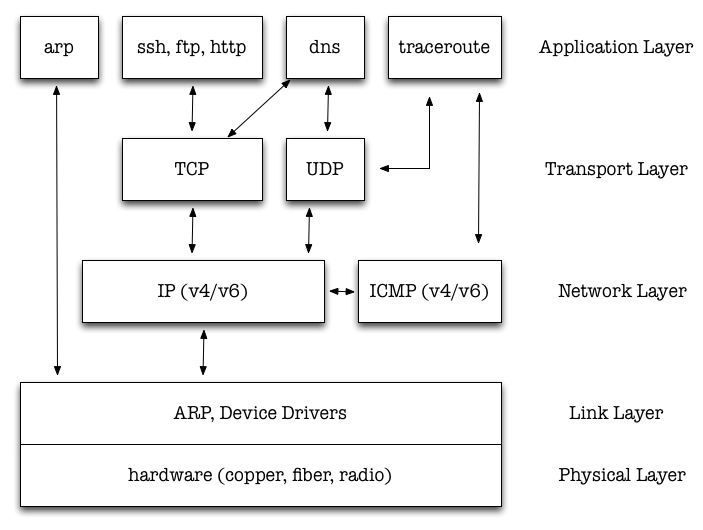
\includegraphics[scale=0.6]{pics/tcpip-stack.eps}
\end{center}
\vspace*{\fill}

\subsection{Networking}
\vspace*{\fill}
\begin{center}
	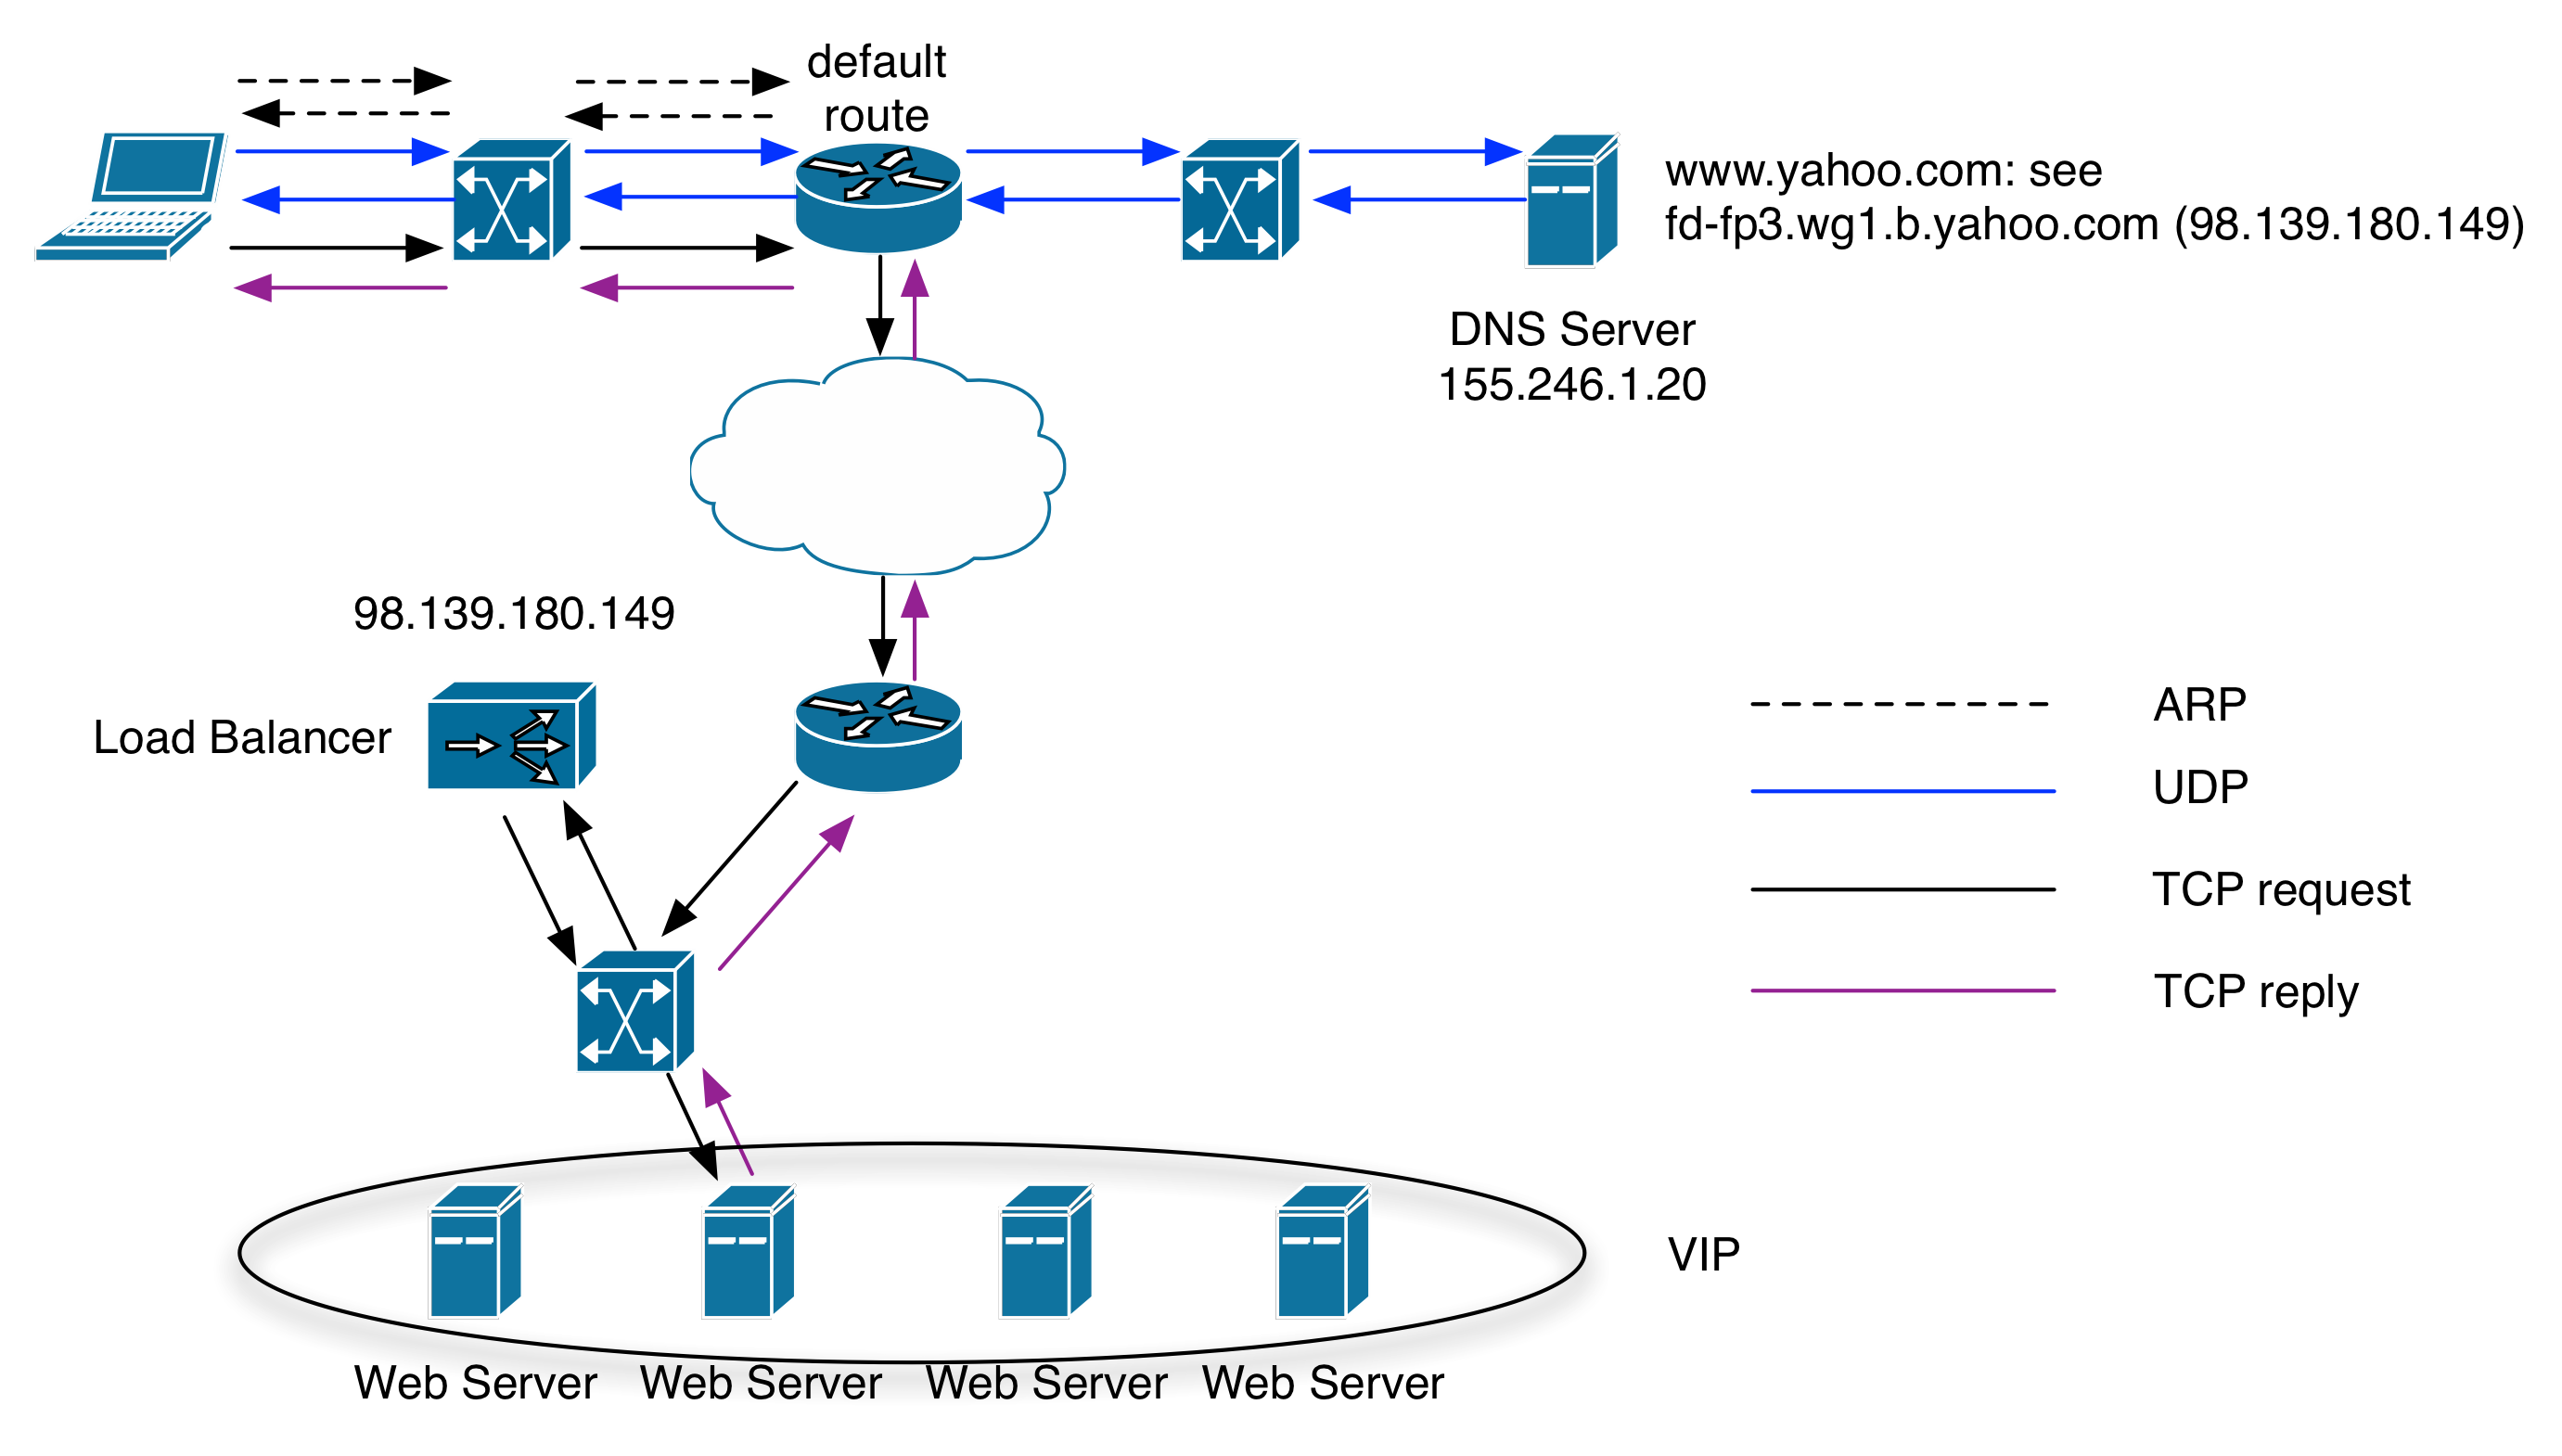
\includegraphics[scale=0.8]{pics/dsr.eps} \\
\end{center}
\vspace*{\fill}

\subsection{Homework}

\verb+https://www.cs.stevens.edu/~jschauma/615/s18-hw4.html+


\subsection{Reading}
\begin{itemize}
	\item \verb+tcpdump(8)+
	\item \verb+ktrace(1)+ / \verb+strace(1)+
	\item \verb+tcp(4)+/\verb+ip(4)+
	\item \verb+netstat(1)+
	\item \verb+nslookup(1)+
\end{itemize}

\end{document}
